\documentclass[tikz,border=8pt]{standalone}
% Shared look for every TikZ diagram. Load with % Shared look for every TikZ diagram. Load with % Shared look for every TikZ diagram. Load with \input{../../tools/tikz-style.tex}
\usepackage[T1]{fontenc}
\usepackage{lmodern}
\renewcommand{\sfdefault}{lmr}  % diagrams use the same serif as the text
\usetikzlibrary{arrows.meta, positioning, shapes.geometric, calc, fit, backgrounds}
\definecolor{cblue}{HTML}{4C78A8}
\definecolor{corange}{HTML}{F58518}
\definecolor{cgreen}{HTML}{54A24B}
\definecolor{cred}{HTML}{E45756}
\definecolor{cpurple}{HTML}{B279A2}
\definecolor{cgrey}{HTML}{6B6B6B}
\tikzset{
  every picture/.style={font=\sffamily, line width=1.2pt},
  box/.style={draw=#1, fill=#1!12, rounded corners=4pt, align=center, inner sep=7pt, minimum height=1.1cm},
  box/.default=cgrey,
  arrow/.style={-{Stealth[length=3mm]}, draw=cgrey, line width=1.4pt},
  title/.style={font=\sffamily\bfseries\Large},
  note/.style={font=\sffamily\small, text=cgrey, align=center},
}
\AtBeginDocument{\hyphenpenalty=10000 \exhyphenpenalty=10000}

\usepackage[T1]{fontenc}
\usepackage{lmodern}
\renewcommand{\sfdefault}{lmr}  % diagrams use the same serif as the text
\usetikzlibrary{arrows.meta, positioning, shapes.geometric, calc, fit, backgrounds}
\definecolor{cblue}{HTML}{4C78A8}
\definecolor{corange}{HTML}{F58518}
\definecolor{cgreen}{HTML}{54A24B}
\definecolor{cred}{HTML}{E45756}
\definecolor{cpurple}{HTML}{B279A2}
\definecolor{cgrey}{HTML}{6B6B6B}
\tikzset{
  every picture/.style={font=\sffamily, line width=1.2pt},
  box/.style={draw=#1, fill=#1!12, rounded corners=4pt, align=center, inner sep=7pt, minimum height=1.1cm},
  box/.default=cgrey,
  arrow/.style={-{Stealth[length=3mm]}, draw=cgrey, line width=1.4pt},
  title/.style={font=\sffamily\bfseries\Large},
  note/.style={font=\sffamily\small, text=cgrey, align=center},
}
\AtBeginDocument{\hyphenpenalty=10000 \exhyphenpenalty=10000}

\usepackage[T1]{fontenc}
\usepackage{lmodern}
\renewcommand{\sfdefault}{lmr}  % diagrams use the same serif as the text
\usetikzlibrary{arrows.meta, positioning, shapes.geometric, calc, fit, backgrounds}
\definecolor{cblue}{HTML}{4C78A8}
\definecolor{corange}{HTML}{F58518}
\definecolor{cgreen}{HTML}{54A24B}
\definecolor{cred}{HTML}{E45756}
\definecolor{cpurple}{HTML}{B279A2}
\definecolor{cgrey}{HTML}{6B6B6B}
\tikzset{
  every picture/.style={font=\sffamily, line width=1.2pt},
  box/.style={draw=#1, fill=#1!12, rounded corners=4pt, align=center, inner sep=7pt, minimum height=1.1cm},
  box/.default=cgrey,
  arrow/.style={-{Stealth[length=3mm]}, draw=cgrey, line width=1.4pt},
  title/.style={font=\sffamily\bfseries\Large},
  note/.style={font=\sffamily\small, text=cgrey, align=center},
}
\AtBeginDocument{\hyphenpenalty=10000 \exhyphenpenalty=10000}

\begin{document}
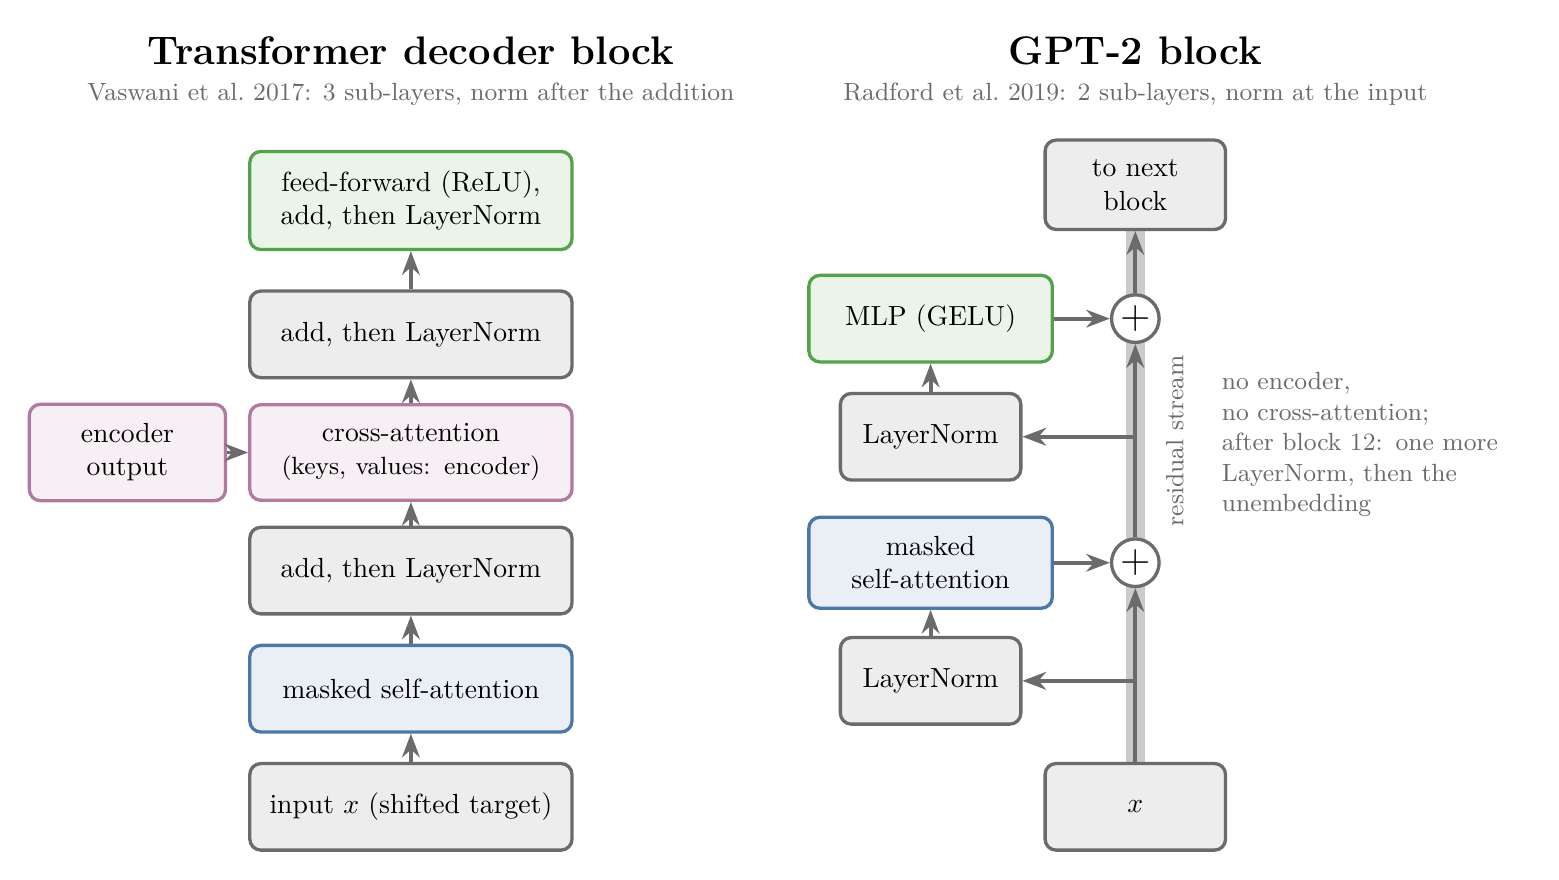
\begin{tikzpicture}[every node/.append style={font=\sffamily}]
  % ---- left: the decoder block of Vaswani et al. 2017 (post-LN, 3 sub-layers) ----
  \node[title] at (0,9.6) {Transformer decoder block};
  \node[note] at (0,9.05) {Vaswani et al.\ 2017: 3 sub-layers, norm after the addition};
  \node[box=cgrey, text width=3.6cm] (in1) at (0,0) {input $x$ (shifted target)};
  \node[box=cblue, text width=3.6cm] (m1) at (0,1.5) {masked self-attention};
  \node[box=cgrey, text width=3.6cm] (n1) at (0,3.0) {add, then LayerNorm};
  \node[box=cpurple, text width=3.6cm] (c1) at (0,4.5) {cross-attention\\\small(keys, values: encoder)};
  \node[box=cgrey, text width=3.6cm] (n2) at (0,6.0) {add, then LayerNorm};
  \node[box=cgreen, text width=3.6cm] (f1) at (0,7.7) {feed-forward (ReLU),\\ add, then LayerNorm};
  \node[box=cpurple, text width=2.0cm] (enc) at (-3.6,4.5) {encoder\\output};
  \draw[arrow] (in1) -- (m1); \draw[arrow] (m1) -- (n1); \draw[arrow] (n1) -- (c1);
  \draw[arrow] (c1) -- (n2); \draw[arrow] (n2) -- (f1); \draw[arrow] (enc) -- (c1);
  % ---- right: GPT-2 block (pre-LN, 2 sub-layers) ----
  \begin{scope}[xshift=9.2cm]
  \node[title] at (0,9.6) {GPT-2 block};
  \node[note] at (0,9.05) {Radford et al.\ 2019: 2 sub-layers, norm at the input};
  \draw[line width=7pt, cgrey!35] (0,-0.4) -- (0,8.1);
  \node[note, rotate=90] at (0.5,4.65) {residual stream};
  \node[box=cgrey, text width=1.8cm] (x) at (0,0) {$x$};
  \node[box=cgrey, text width=1.8cm] (l1) at (-2.6,1.6) {LayerNorm};
  \node[box=cblue, text width=2.6cm] (a) at (-2.6,3.1) {masked\\self-attention};
  \node[circle, draw=cgrey, fill=white, inner sep=1pt, font=\Large] (p1) at (0,3.1) {$+$};
  \node[box=cgrey, text width=1.8cm] (l2) at (-2.6,4.7) {LayerNorm};
  \node[box=cgreen, text width=2.6cm] (f) at (-2.6,6.2) {MLP (GELU)};
  \node[circle, draw=cgrey, fill=white, inner sep=1pt, font=\Large] (p2) at (0,6.2) {$+$};
  \node[box=cgrey, text width=1.8cm] (y) at (0,7.9) {to next block};
  \draw[arrow] (x.north) |- (l1); \draw[arrow] (l1) -- (a); \draw[arrow] (a) -- (p1);
  \draw[arrow] (p1.north) |- (l2); \draw[arrow] (l2) -- (f); \draw[arrow] (f) -- (p2);
  \draw[arrow] (x) -- (p1); \draw[arrow] (p1) -- (p2); \draw[arrow] (p2) -- (y);
  \node[note, text width=3.8cm, align=left] at (3.0,4.6) {no encoder,\\no cross-attention;\\after block 12: one more\\LayerNorm, then the\\unembedding};
  \end{scope}
\end{tikzpicture}
\end{document}
